% Author: Izaak Neutelings (June 2020)
% Inspiration: https://tex.stackexchange.com/questions/285578/how-to-draw-parallelepiped-and-cube-with-latex/288101#288101
\documentclass[border=3pt,tikz]{standalone}
\usepackage{amsmath}
\usepackage{physics}
\usepackage{siunitx}
\usepackage{xcolor}
\usepackage{etoolbox} %ifthen
\usepackage[outline]{contour} % glow around text
%\usetikzlibrary{arrows,arrows.meta}
%\usetikzlibrary{calc}
%\usetikzlibrary{decorations.markings}
%\usetikzlibrary{angles,quotes} % for pic (angle labels)
\tikzset{>=latex} % for LaTeX arrow head
\contourlength{1.6pt}

\colorlet{myblue}{blue!70!black}
\colorlet{mydarkblue}{blue!40!black}
\colorlet{mygreen}{green!60!black}
\colorlet{myred}{red!65!black}
\colorlet{mypurple}{red!50!blue!95!black!75}
\colorlet{xcol}{blue!85!black}
\colorlet{vcol}{green!70!black}
\colorlet{projcol}{vcol!90!black!60}
\tikzstyle{wave}=[myblue,thick]
\tikzstyle{xline}=[very thick,myblue]
%\tikzstyle{vline}=[very thick,mygreen]
%\tikzstyle{aline}=[very thick,mypurple]
\tikzstyle{vector}=[->,very thick,vcol,line cap=round]
\tikzstyle{mydashed}=[green!30!black!90,dash pattern=on 2pt off 2pt,very thin]
\tikzstyle{mymeas}=[{Latex[length=3,width=2]}-{Latex[length=3,width=2]},thin]
\def\tick#1#2{\draw[thick] (#1) ++ (#2:0.05*\ymax) --++ (#2-180:0.1*\ymax)}


\begin{document}



% POSITION - PARABOLA + slopes
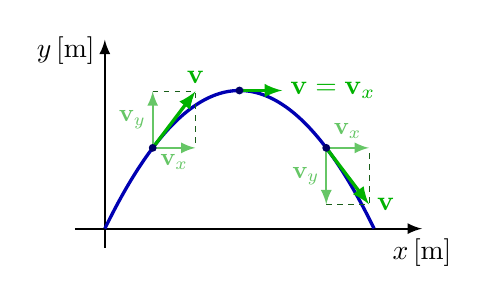
\begin{tikzpicture}
  \def\slope{0.65}
  \def\xmax{3.8}
  \def\ymax{2.4}
  \def\A{0.6}
  \def\v{0.9}
  \def\xa{0.16*\xmax}
  \def\xm{0.45*\xmax}
  \def\xb{0.74*\xmax}
  \def\ya{\A*(\root-\xa)*\xa}
  \def\ym{\A*(\root-\xm)*\xm}
  \def\root{0.9*\xmax}
  \def\nsamples{100}
  \def\ang{atan(\A*(\root-2*\xa))}
  \def\vx{{\v*cos(\ang)}}
  \def\vy{{\v*sin(\ang)}}
  \coordinate (A) at (\xa,{\ya});
  \coordinate (M) at (\xm,{\ym});
  \coordinate (B) at (\xb,{\ya});
  
  \draw[->,thick]
    (-0.1*\xmax,0) -- (1.06*\xmax,0) node[below] {$x$\,[m]};
  \draw[->,thick]
    (0,-0.1*\ymax) -- (0,\ymax) node[below=4,left=0] {$y$\,[m]};
  \draw[xline,variable=\t,samples=\nsamples,smooth,domain=0:\root]
    plot(\t,{\A*(\root-\t)*\t}); %node[right=7,above=-2] {$x=x(t)$};
  
  % VECTOR A
  \draw[->,vcol,very thick]
    (A) --++ ({\ang}:\v) coordinate (VA) node[above=-1] {$\vb{v}$};
  \draw[mydashed]
    (A) ++ (0,\vy) -- (VA) --++ (0,-\vy);
  \draw[<->,projcol,thick]
    (A) ++ (0,\vy) -- (A) node[scale=0.9,midway,left=-1] {$\vb{v}_y$}
      --++ (\vx,0) node[scale=0.9,midway,below=-1] {$\vb{v}_x$};
  
  % VECTOR M
  \draw[->,vcol,very thick]
    (M) --++ (\vx,0) node[right=-1] {$\vb{v} = \vb{v}_x$};
  
  % VECTOR B
  \draw[->,vcol,very thick]
    (B) --++ ({-\ang}:\v) coordinate (VB) node[right=-1] {$\vb{v}$};
  \draw[mydashed]
    (B) ++ (0,-\vy) -- (VB) --++ (0,\vy);
  \draw[<->,projcol,thick]
    (B) ++ (0,-\vy) -- (B) node[scale=0.9,midway,left=-1] {$\vb{v}_y$}
      --++ (\vx,0) node[scale=0.9,midway,above=] {$\vb{v}_x$};
  
  % POINTS
  \fill[mydarkblue]
    (A) circle (0.05)
    (M) circle (0.05)
    (B) circle (0.05);
  
\end{tikzpicture}



\end{document}